
\chapter{Benchmark Results}\label{chap:benchmarks}
We have compared the performance of the conjugate gradient solver provided via the {\MATLAB} interface of {\ViennaCL} with the built-in functions of {\MATLAB}. The code used for the benchmarks can be found in the files \texttt{test\_cg.m}.

\begin{center}
\begin{tabular}{|l|l|}
\hline
CPU & Intel Core i7 960 \\
GPU & NVidia Geforce GTX 470 \\
RAM & 6 GB \\
OS  & Windows 7 Ultimate, 32 bit \\
Nvidia driver version: & 197.75 \\
{\ViennaCL} version  & 1.0.2 \\
\hline
\end{tabular}
\end{center}

\NOTE{Compute kernels are not fully optimized yet, results are likely to improve considerably in future releases of {\ViennaCL}}

\begin{figure}[tbp]
    \centerline{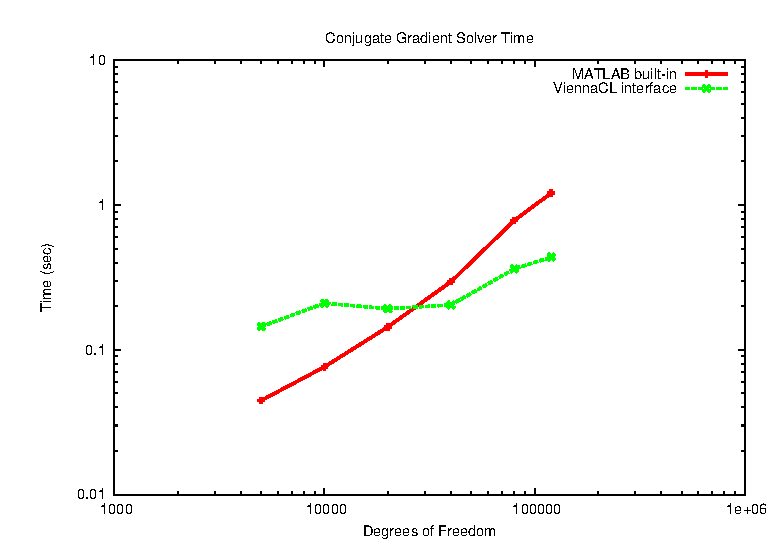
\includegraphics[width=0.9\textwidth]{figures/cg-matlab}}
    \caption{Execution time for ten conjugate gradient solver runs (27 iterations each) for different problem sizes. }
    \label{fig:matlab-cg}
\end{figure}

The results in Fig.~\ref{fig:matlab-cg} show that there is a certain overhead related to starting the compute kernels in {\OpenCL}. However, for large systems, this overhead becomes negligible and the performance benefit can readily be seen. 